%%%%%%%%%%%%%%%%%%%%%%%%%%%%%%%%%%%%%%%%%%%%%%%%%%%%%%%%%%%%%%%%%%
\section{Limitations}\label{sec:limitations}
%%%%%%%%%%%%%%%%%%%%%%%%%%%%%%%%%%%%%%%%%%%%%%%%%%%%%%%%%%%%%%%%%%
% Stream feeding this section: R7 (foilInWind), with B1 (solid-block
% preconditioner) and B2 (collapsibleChannel solid resolution).

This section reports where the method, as implemented and released, is limited: a case in which the time step must be reduced for Newton to converge, the treatment of the solid block in the preconditioner, the accuracy of the velocity solid on thin structures, and the software on which the implementation runs.

%%--------------------------------------------------------------------------------------------------------------------%%
\subsection{Time-step limit in a three-dimensional flag}\label{sec:lim_foil}
% TIME-SCHEME NOTE (Philip, 22 Oct 2026), for anyone adding results here:
% all transient results in this paper must use BDF2 (backward) for the fluid
% ddt(U) and the solid. The solids4foam tutorial default for this case is
% backward for the fluid ddt(U). Confirm and record the ddt schemes of every
% run (runs.csv); rerun any result computed with Euler, and say so here.
% Every run here: fluid ddt(U), ddt(dU), ddt(p) and solid backward (runs.csv, tutorial).
%%--------------------------------------------------------------------------------------------------------------------%%
% Set-up: solids4foam origin/fix/foilInWind-monolithic-timestep @ b157ecaf3
% (solids4foam PR #602), tutorials/fluidSolidInteraction/foilInWind/README.md
% and system/controlDict.monolithic (dt = 0.0025 s); case summary from A1
% Section 1.10. The README cites no benchmark; the flapping "has not been
% verified".

A thin flexible foil attached behind a rigid block in a uniform air stream (Figure~\ref{fig:foil_geom_m}) undergoes a three-dimensional flapping motion.
The block is $1\,\mathrm{cm}$ square in cross-section and $3\,\mathrm{cm}$ long; the foil is $4\,\mathrm{cm}$ long, $3\,\mathrm{cm}$ wide and $0.6\,\mathrm{mm}$ thick, a St Venant--Kirchhoff solid with $E = 2\,\mathrm{MPa}$ and $\rho_s = 2000\,\mathrm{kg/m^3}$, in air at $1\,\mathrm{m/s}$.
The fluid mesh has 176\,248 cells and the solid mesh $32\times6\times24$ cells.
No reference solution exists; the case is used to compare the time step and cost needed by the two couplings.

\begin{figure}[htbp]
	\centering
	\includegraphics[scale=1]{figures/foilInWind-geometry}
	\caption{Flexible foil behind a rigid block: geometry and base mesh in side and top view (dimensions in cm).}
	\label{fig:foil_geom_m}
\end{figure}

\paragraph{Measured.}
Both couplings are run to $t = 0.2\,\mathrm{s}$, through the start-up, with $\Delta t = 0.01$, $0.005$ and $0.0025\,\mathrm{s}$; IQN-ILS uses the strict convergence test with the tutorial tolerance of $10^{-5}$ and at most 50 coupling iterations, and the quasi-monolithic coupling the tutorial Newton tolerance of $10^{-4}$, a backtracking line search and at most 50 Newton iterations.
Adaptive time stepping, which the implementation provides, is off in every run.
The cost is compared at $\Delta t = 0.005\,\mathrm{s}$ on the same eight processes of one workstation.
% QM: evidence/m-runs-a-rfix 7a (1252bd2e5, 128 ranks, MeluXina); IQN-ILS:
% evidence/m-runs-a 7a (85b0c1de6, 8 ranks); equal-rank pair: local Mac
% Studio, a421f063d-equivalent build, ~/claude-runs/agent-b-foil (1 Nov 2026).

\begin{figure}[htbp]
	\centering
	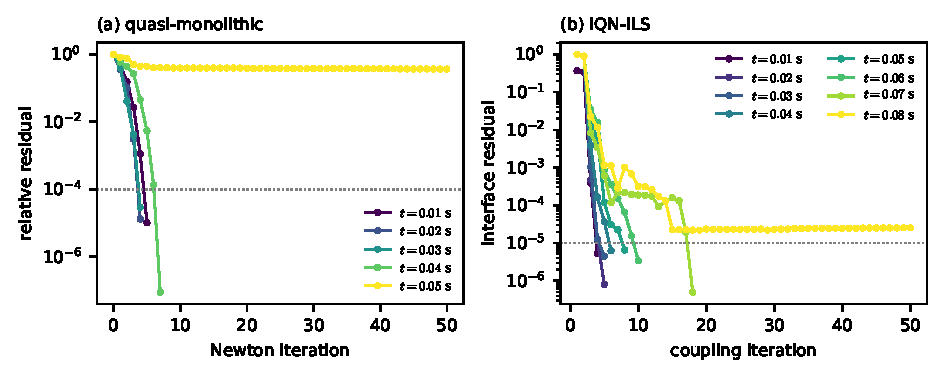
\includegraphics[width=\textwidth]{figures/foilInWind-stall}
	\caption{Flexible foil behind a rigid block, $\Delta t = 0.01\,\mathrm{s}$: (a) Newton residual of the quasi-monolithic coupling relative to its value at the start of each step, and (b) interface residual of IQN-ILS, against the iteration count, for each step until the run stops; dotted: tolerance.}
	\label{fig:foil_stall}
\end{figure}

\paragraph{Results.}
With $\Delta t = 0.01\,\mathrm{s}$ neither coupling completes the start-up (Figure~\ref{fig:foil_stall}).
The Newton iteration needs 4 to 5 iterations in the first three steps and 7 in the fourth, and in the fifth, at $t = 0.05\,\mathrm{s}$, the residual falls to $37\%$ of its initial value within about 15 iterations and then stagnates, with the line search shortening the step, until the iteration limit is reached.
The coupling iterations of IQN-ILS grow in the same way, 4, 5, 5, 6, 8, 10 and 18 in the first seven steps, and at $t = 0.08\,\mathrm{s}$ the interface residual stagnates at $2.5\times10^{-5}$, above the tolerance, for the remaining iterations.
Right preconditioning, unlimited convection and other differencing parameters of the matrix-free product stall in the same way, so the stagnation of Newton is attributed to the nonlinearity of the coupled problem over a large step rather than to the linear solver; that IQN-ILS fails at nearly the same time supports this.
With $\Delta t = 0.005\,\mathrm{s}$ both couplings complete, the quasi-monolithic coupling with 3.3 Newton iterations per step (at most 4) and 36 Krylov iterations per Newton iteration, and IQN-ILS with 5.4 coupling iterations per step (at most 8); on eight processes the quasi-monolithic run takes $337\,\mathrm{s}$ and the IQN-ILS run $229\,\mathrm{s}$, 1.5 times less.
With $\Delta t = 0.0025\,\mathrm{s}$ the counts fall to 2.9 Newton and 4.7 coupling iterations per step.
On this case, with a dense solid ($\rho_s/\rho_f \approx 1700$) and therefore little added mass, the quasi-monolithic coupling brings no gain in robustness and costs more per step than IQN-ILS.
The method has no globalisation beyond a backtracking line search; adaptive time stepping on Newton failure, or a continuation method, may let it pass such start-ups automatically, but neither is assessed here.

%%--------------------------------------------------------------------------------------------------------------------%%
\subsection{Solid block of the preconditioner}\label{sec:lim_solid_pc}
%%--------------------------------------------------------------------------------------------------------------------%%
% Background: campaign/HANDOFF.md B1; A4 Section 6; method section
% (origin/manuscript/d1-method) Section "Field-split preconditioner".
% Historical (April 2026, commit 2f99ea065): per-process bjacobi+LU on the
% solid block changed the foilInWind solid response with the process count;
% a preconditioner must not change a converged answer, so the Newton
% tolerance was too loose then. Not reported (the acceptance test of check B1
% now guards against it).

% Check B1: evidence/campaign-g1:paper-data/campaign/b1/findings.md
% (solids4foam 257b2e564; ring factor 2 moderate, cavity L3, 3dTube L2).
In the two-dimensional cases of this paper, the solid block of the preconditioner is factorised exactly with a sparse LU factorisation, of which every process holds a complete copy.
This is robust, and affordable because the solid block is small compared with the fluid block in these cases, but its cost and memory do not fall with the process count and grow with the size of the solid.
On level 2 of the three-dimensional tube the factorisation takes the same time on 16 processes as on 4, with its memory growing from 9 to 25\,GB, and one V-cycle of BoomerAMG is 4 and 12 times faster on 4 and 16 processes at the same Newton and Krylov iteration counts; it is therefore used for the tube (Sections~\ref{sec:tube3d_pc_study} and~\ref{sec:tube3d_scaling}).
On the small solid blocks of the two-dimensional cases the exact factorisation remains the cheaper choice: BoomerAMG doubles the Krylov iterations on the ring and costs 1.4--1.9 times as much, and on the cavity it costs 10--14\% more.
With either preconditioner the converged solution agrees with a run converged to a hundred times tighter Newton tolerances to within $7\times10^{-5}$ of each monitored quantity, relative to its largest magnitude and close to the output resolution of the monitors, so the choice affects cost only.
An algebraic multigrid solid block for thin, nearly incompressible or strongly nonlinear solids has not been assessed.

%%--------------------------------------------------------------------------------------------------------------------%%
\subsection{Velocity solid on thin structures}\label{sec:lim_thin_solid}
%%--------------------------------------------------------------------------------------------------------------------%%
% Source: companion paper sectionBenchmarkSuite.tex, "Collapsible channel"
% (Solid bullet) and "Ring added-mass problem" (Solid discretisation bullet);
% collapsibleChannel/verification/README.md "Quasi-monolithic coupling".
% The high-order (MLS) solid is not available for velocity solids and will
% not be added for this paper (Philip's decision).

The velocity solids use the standard second-order cell-centred discretisation with linear reconstruction.
For thin, bending-dominated structures meshed with few, elongated cells across the thickness, this discretisation is too stiff: in the companion paper, the same discretisation of the collapsible-channel wall in a static test is between $16.7\%$ and $0.22\%$ too stiff over the solid meshes used there, whereas a high-order reconstruction is within $0.25\%$ on every mesh~\citetodo{companion verification paper}.
The high-order reconstruction is not available for the velocity solids, so the accuracy of the quasi-monolithic coupling on such cases is limited by the solid unless the solid is refined along its length; with a non-conformal interface the solid can be refined independently of the fluid (Section~\ref{sec:robustness_collapsible}): on the collapsible channel a $640\times8$ solid coupled through AMI to fluid level 2 brings the first trough to within $0.71\%$ of the oomph-lib reference in about a third of the wall time of the conformal $320\times8$ solid on fluid level 4, whose trough lies $1.17\%$ from it.
% B2: evidence/m-runs-b:paper-data/campaign/wp3/b2_618/ (3823 s against 11080 s, shared XenoSim node, indicative).
The wet/dry frequency ratio of the ring problem is insensitive to this error, because the wet and dry runs share it (Section~\ref{sec:ring_m}).

%%--------------------------------------------------------------------------------------------------------------------%%
\subsection{Fluid mesh motion}\label{sec:lim_mesh_motion}
%%--------------------------------------------------------------------------------------------------------------------%%

The fluid mesh is moved once per step to a displacement extrapolated from the solid (Section~\ref{sec:fluid_mesh_motion}), outside the Newton system, so its robustness is that of the mesh-motion solver rather than of the coupled iteration.
Two failures of the mesh motion occurred in the campaign, and both were removed by changing the mesh-motion set-up, not the coupling.
On the collapsible channel at the largest time step, the first iterate of the nonlinear pseudo-solid carried the whole wall increment of a step into the half-cells next to the wall and stopped the mesh-motion solve, while the coupled Newton iteration still converged in three iterations per step; extrapolating the first iterate in time removed the failure (Section~\ref{sec:robustness_collapsible}).
On the refined Hron--Turek meshes, whose first cells at the flag tip are $0.3\,\mathrm{mm}$ thick, a Laplacian mesh motion solved incrementally on the moving mesh inverted cells near the tip within the first second of a replayed flag motion on levels 2 to 4, whereas each step solved separately from the initial mesh, with a linear inverse-distance stiffness, kept every cell valid; the error of the incremental solve accumulates with the motion.
A linear elastic pseudo-solid with a linear inverse-distance stiffness (Section~\ref{sec:fluid_mesh_motion}) keeps every cell valid: assembled on the initial mesh, it moves levels 2 to 4 through $5.2\,\mathrm{s}$ of replayed flag motion, about 28 periods, with a largest non-orthogonality of $39$--$45^\circ$, close to that of the initial meshes; assembled on the current mesh, the form used in the coupled runs of Section~\ref{sec:fsi3_m} because the partitioned couplings accept only that form, it moves levels 2 and 3 past the times at which the Laplacian motion failed with no invalid cell.
Neither failure involves the coupled residual, but both show that a quasi-monolithic method that moves the mesh outside its Newton system inherits the limits of its mesh-motion solver, which must be chosen for the largest interface increment per step and the smallest cells next to the interface.
% FSI3 motion gate: ~/claude-runs/agent-b-gmsh/work/tlg_{2,3,4}, board 6549050077
% and 6551325237 (1 Nov 2026); meshes t1-t4 from ht_mesh_gmsh2.py --tip-y1 3e-4.

%%--------------------------------------------------------------------------------------------------------------------%%
\subsection{Software}\label{sec:lim_platform}
%%--------------------------------------------------------------------------------------------------------------------%%
% Source: A3 Section 4 (paper-data/a3_pr233_merge_readiness.md): the coupler
% source is inside #ifdef USE_PETSC / #ifdef OPENFOAM_COM; CI on 257b2e564
% builds OpenFOAM v2312, v2412, v2512, OpenFOAM-9 and foam-extend-4.1, with and
% without PETSc; the monolithic tutorials stop on OpenFOAM.org and
% foam-extend.

The quasi-monolithic coupling requires the OpenFOAM.com (ESI) line of OpenFOAM and PETSc; solids4foam builds without it on the other OpenFOAM lines and without PETSc.
% MeluXina builds (qm-head, qm-a421): OpenFOAM-v2512, foss/2024a (GCC 13.3),
% PETSc 3.22.0, hypre 2.31.0; XenoSim build (wp3 3b runs): GCC 11.4, PETSc
% 3.24.1, hypre 2.33.0 (runs.csv); workstation (macOS, Clang): PETSc 3.22.2.
The results of this paper were obtained with OpenFOAM v2512 and PETSc 3.22 or 3.24; the coupling also builds with OpenFOAM v2312 and v2412 with PETSc.
The partitioned couplings with which it is compared are available on all supported OpenFOAM lines.

\paragraph{Scope and modularity.}
Partitioned coupling in solids4foam combines any of its fluid and solid models, including displacement-based solids with high-order reconstruction, and runs on every supported OpenFOAM line~\citep{Tukovic2018, Cardiff2025}.
The quasi-monolithic coupling is restricted to the coupled Newton fluid model of solids4foam (\texttt{newtonIcoFluid}) and the velocity solids (Section~\ref{sec:numerical_methods}), to the OpenFOAM.com line with PETSc (Section~\ref{sec:lim_platform}), and to the standard second-order solid reconstruction, which limits its accuracy on thin structures (Section~\ref{sec:lim_thin_solid}).
A new physical model enters the quasi-monolithic coupling only with its contribution to the residual and to the approximate Jacobian, whereas it enters partitioned coupling through its interface data alone.
Where both couplings apply, the choice is thus between a solver that converges independently of the added mass at a higher cost per iteration, and a modular solver whose cost and reliability depend on the added mass and on its acceleration settings.
